\documentclass[titlepage]{article}
\usepackage{amsmath, amssymb}
\usepackage{minted}
\usepackage{graphicx}
\usepackage{tikz}
\usepackage[colorlinks=true]{hyperref}


\newmintinline[cinline]{c}{}
\newcommand{\N}{\mathbb{N}}
\newcommand{\R}{\mathbb{R}}
\newcommand{\I}{\mathbb{I}}
\renewcommand{\S}{\texttt{S}}
\newcommand{\xuniform}{\ensuremath{X_{\texttt{uniform}}}}
\newcommand{\zo}{\{0, 1\}}
\newcommand{\uniformbool}{\texttt{uniformbool}}
\newcommand{\p}{\mathbf{p}}
\newcommand{\q}{\mathbf{q}}

\newcommand{\E}[1]{\mathbb{E}\left[ #1 \right]}

\newcommand{\m}{\mathbf{m}}
\renewcommand{\P}{\mathfrak{P}}
\newcommand{\Prop}{\texttt{Prop}}
\newcommand{\M}{\mathfrak{M}}
\newcommand{\K}{\mathfrak{K}}
\newcommand{\qed}{\ensuremath{\triangle}}

\newtheorem{theorem}{Theorem}
\newtheorem{proof}{Proof}[theorem]
\title{Markov Chain Monte Carlo:  Metropolis-Hastings \& Hamiltonian Monte Carlo }
\author{Siddharth Bhat (20161105) ~ \texttt{siddu.druid@gmail.com}}
\date{\today}
\begin{document}
\maketitle

\section{Introduction}

All the code for this project (including code to generate the report and
its graphs) can be found at \url{https://github.com/bollu/sampleraytracer}.

% Consider that we are plonked down in the \texttt{C } programming language, and
% our only method to generate random numbers is to call \cinline{int rand(void)}.
% However, \emph{the type is a lie}, since we are able to modify global mutable
% state. So, really, to have a mathematical discussion about the whole state
% of affairs, we will write the type of \cinline{rand} as
% $\cinline{rand}: S \rightarrow S \times \cinline{int}$ --- that is,
% it receives the entire state of the program, and then returns the \cinline{int},
% along with the new state of the program.
% $\uniformbool: \S \rightarrow \S \times \zo$.
% 
% When we say that \texttt{rand} generates random numbers, we need to be a
% little more specific: what does it mean to generate random numbers? we need to
% describe the \emph{distribution} according to which we are receiving the random
% numbers from the random number generator $rand$.  What does that mean?
% Well, it means that as we generate more numbers, the \emph{empirical distribution}
% of the list of numbers we get from the successive calls to $\uniformbool$ tends
% to some \emph{true distribution}. We will call this \emph{true distribution}
% succincty as \textbf{the} distribution of the random number generator. Formally,
% let us define $F(t) \equiv \int_0^t P(x) dx$ to be the cumulative distribution 
% of $P$.
% 
% In the case of 
% $\uniformbool$, we are receiving random numbers according to the distribution:
% $$
% P_{\uniformbool}: \zo \rightarrow [0, 1]; \qquad P_{\uniformbool}(x) = 1/2
% $$
% That is, both $0$ and $1$ are \emph{equally likely}. However, this is
% extremely boring. What we are \emph{usually} interested in is to sample $\{0, 1\}$
% in some \emph{biased} fashion:
% $$
% P_{\uniformbool}^{bias}: \zo \rightarrow [0, 1]; 
% \qquad P_{\uniformbool}^{bias}(0) = bias;
% \qquad P_{\uniformbool}^{bias}(1) = 1 - bias
% $$
% 
% And far more generally, we want to sample from \emph{arbitrary domains} with
% \emph{arbitrary distributions}:
% 
% $$
% \texttt{sampler}_X^P: S \rightarrow S \times X; 
% $$
% 
% This function is boring. What we \emph{really} want to sample from are
% more interesting distributions. For example:
% 
% \begin{itemize}
%     \item The normal distribution $P(x: \R) = e^{-x^2}$.
%     \item The poisson distribution $P(x: \N) = e^{-\lambda} \lambda^n/n!$.
%     \item A custom distribution $P(x: \R) = |sin(x)|$.
% \end{itemize}

\subsection{MCMC sampling: the fundamental algorithm}

markov-chain-monte-carlo methods are a class of algorithms which blend together
two or three properties; these properties blend together in subtle ways,
and permit us to solve very different-looking-problems using the same toolkit,
by leveraging different portions of the algorithm's power. Broadly, they
all solve the following problem:

\begin{quote}
    Given an \textbf{arbitrary} function $\P: X \rightarrow \R$, \textbf{create a sampler} for the
    \textbf{normalized} probability distributed from $\P$, $\hat \P(x) \equiv \frac{\P(x)}{\int \P(x) dx}$.
    Furthermore, allow the sampling process to be \textbf{guided by} a proposal distribution:
    $\Prop: X \rightarrow (X \rightarrow [0, 1])$. This proposal, for each
    location $x_0 \in X$, permits the specification of a '\textbf{likely direction} of higher likelihood',
    $\Prop(x_0): X \rightarrow \R$.
\end{quote}

\subsection{Sampling use case 1. Simulation And Sampling}
Often, we do really want samples from a particular distribution. For example,
we might often want to apply Bayes' rule and sample from the posterior
distribution. Assume that we have a computational procedure to compute
$P(X=x_0|Y=y_0)$. We now want to $P(Y|X=x_0)$.

$$
P(Y|X=x_0) = \frac{P(X=x_0|Y)P(Y)}{\sum_{y} P(X=x_0|Y=y)}
$$

There are two problems in sampling the above distribution:
\begin{itemize}
    \item[1] The expression $P(Y=y|X=x)$ has no a-priori structure. Hence,
        we will need an algorithm that can sample from an arbitrary distribution.
    \item[2] The denominator term, which is a normalization factor can
        be extremely expensive to compute due to the summation involved
\end{itemize}

Hence, we need to use MCMC to sample from $P(Y|X=x_0)$, and we can
expedite this by sampling from $\P(Y|X=x_0) = P(X=x_0|Y)P(Y) \propto P(Y|X=x_0)$


\subsection{Sampling use case 2. Gradient Free Optimisation}
We  want to maximize a function $f: X \rightarrow \R$. However, we lack
gradients for $f$, hence we cannot use techniques such as gradient
descent, or other techniques from convex optimisation.
In such a case, we can consider $f$ as some sort of unnormalized
probability distribution, and use MCMC to sample from $f$.

That is, we set $\P \equiv f$. Now, samples from $\P$ will be 'more likely'
to come from those regions where $f$ is large, since a sampler
will be more likely to sample from regions of high probability.


\subsection{Sampling use case 3. Numerical Integration}

We wish to calculate $\int_l^u f(x) dx$ where $f$ is some complicated 
function with no closed form for the definite integral of $f$. In this case,
we know that the average value of a function, denoted by $\E{f}$, can be
computed as:

$$
\E{f} \equiv \frac{1}{|u - l|} \int_l^u f(x) dx
$$

On rearrangement, we get:

$$
\int_l^u f(x) dx = |u - l| \E{f}
$$

Hence, if we have a good approximation of $\E{f}$, we have a good approximation
for the integration. The naive approximation of $\E{f}$ can be found by using:

$$
\E{f} \simeq \frac{1}{n} \sum_{i=1}^n f(x_i)
$$

However, we often know \emph{something} about $f$, just not its \emph{precise} shape:
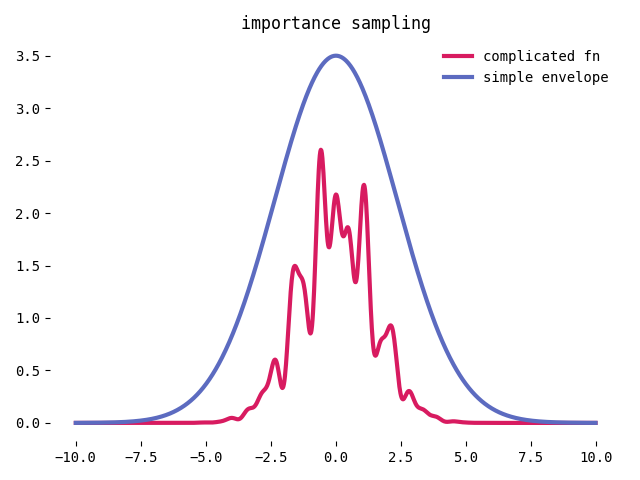
\includegraphics[width=\textwidth]{complicated-fn-simple-envelope.png}

In this case, we can \emph{guide} the sampling process, by setting the proposal
\Prop~as the envelope of the function $f$. That way, we will be more likely
to pick up \emph{useful samples}, which rapidly sample from the region of
space that has mass for the integration.



\section{Where it all begins: The Metropolis Hastings sampler}
\subsection{The big idea}
We wish to sample from a distribution $\P$, but we do not know how to do so.
The idea is that we build a markov chain $M[\P, \Prop]$ where $\P, \Prop$ are
supplied by the user. We will show that the \emph{stationary distribution} of $M[\P, \Prop]$
is going to be $\P$. This will ensure that if we interpret \emph{states of $M$} as samples,
these samples will the distriubted according to $\P$.

\subsection{Detail balance: A tool for proofs}
We will first require a condition that will enable to rapidly establish that some
distribution $\P: X \rightarrow \R$ is the stationary distribution of a markov chain $M$. If
the transition kernel $K: X \times X \rightarrow \R$ of $M \equiv (X, K)$ is such that:

$$
\forall x, x' \in X, \P(x) K(x, x') = \P(x') K(x', x)
$$

Then $\P$ is said to be \textbf{detail balanced} with respect to $M$.

\begin{theorem}
If $\P$ is detail balanced to $M \equiv (X, K: X \rightarrow (X \rightarrow [0, 1])$,
then $\P$ is the stationary distribution of $M$.
\end{theorem}
\begin{proof}
Let $\P$ be detail balanced to $M$. This means that:
$$
\forall x, x' \in X, \P(x) K(x)(x') = \P(x') K(x')(x)
$$

Let us say say that we are in state $\P$. We wish the find the probability
distribution after one step of transition. The probability of being
in some state $x'_0$ is going to be:

$$
Pnext(x'_0) \equiv \sum_x \P(x) K(x)(x'_0)
$$

since we have $\P(x)$ probability to be at a given $x$, and
$K(x, x'_0)$  probability to go from $x$ to $x'_0$. If we add over all possible
$x \in X$, we get the probability of all states to enter in $x'_0$.
Manipulating $Pnext$, we get:

\begin{align*}
&Pnext(x'_0) \equiv \sum_x \P(x) K(x)(x'_0) \\
&= \sum_x \P(x'_0) K(x'_0)(x) \quad \text{(by detail balance)} \\
&= \P(x'_0) \sum_x K(x'_0)(x) \quad \text{($P(x_0)$ is constant} \\
&= \P(x'_0) \cdot 1 \quad \text{($K(x'_0)$ is a distribution which is being summed over)} \\
&= \P(x'_0) \quad \text{(eliminate multiplication with 1)}
\end{align*}

Hence, $Pnext(n'_0) = \P(x'_0)$ if $\P$ is the current state, and $\P$
is in detail balance with the kernel $K$.
This means that $\P$ is the stationary distribution of $M$.
\qed
\end{proof}

\subsection{Metropolis Hastings}

There are three key players in the metropolis hasting sampler:
\begin{itemize}
    \item [1] $\P: X \rightarrow \R$: the probability distribution we wish to sample from.
    \item[2] $\Prop: X \rightarrow (X \rightarrow \R)$. For each $x_0 \in X$,
        provide a distribution $\Prop(x): X \rightarrow \R$ that is used to
        sample points around $x_0$.  $\Prop$ for \emph{proposal}.
    \item [3] $M[\P, \Prop] \equiv (X, K[\P, \Prop]: X \rightarrow \R)$: The
        Metropolis Markov chain we will sample from, whose stationary distribution is $\P$ ---
        $M$ for \emph{Markov}.
\end{itemize}

We want the stationary distribution of $M[\P, \Prop]$ to be $\P$. We also
wish for $K[\P, \Prop](x_0) \sim \Prop(x_0)$: That is, at a point $x_0$, we want
to choose new points in a way that is 'controlled' by the proposal distribution
$\Prop(x_0)$, since this will allow us to 'guide' the markov chain towards regions where $\P$ is high.
If we had a gradient, then we could use $\P'$ to 'move' from the current point
$x_0$ to a new point. Since we lack a gradient, we will provide a custom
$\Prop(x_0)$ for each $x_0$ that will tell us how to pick a new $x'$, in
a way that will improve $\P$.  So, we tentatively define
$$K[\P, \Prop](x)(x') \stackrel{?}{\equiv} \Prop(x)(x').$$

Recall that for $\P$ to be a stationary distribution of $K$, it is sufficient
for $\P$ to be in detail balance for $K$. So, we write:

\begin{align*}
&\P(x) K(x, x') \stackrel{?}{=}  \P(x') K(x', x) \quad \text{(going forward equally likely as coming back)} \\
&\P(x) Prop(x)(x') \stackrel{?}{=} \P(x') Prop(x')(x) \quad \text{(this is a hard condition to satisfy)}
\end{align*}

This is far too complicated a condition to impose on $Prop$ and $\P$, and there
is no reason for this condition to be satisfied in general. Hence,
we add a custom "fudge factor" $\alpha \in X \rightarrow (X \rightarrow \R)$
that tells us how often to transition
from $x$ to $x'$. We redefine the kernel as:

$$
K[\P, \Prop](x)(x') \equiv \Prop(x)(x') \alpha(x)(x')
$$

Redoing detail balance with this new $K$, we get:

\begin{align*}
&\P(x) K(x, x') \stackrel{?}{=}  \P(x') K(x', x) \quad \text{(going forward equally likely as coming back)} \\
&\P(x) Prop(x)(x') \alpha(x)(x') = \P(x') Prop(x')(x) \alpha(x')(x) \quad \text{(Fudge a hard condition with $\alpha$)} \\
&\frac{\alpha(x)(x')}{\alpha(x')(x)} = \frac{\P(x') Prop(x)(x') }{\P(x) Prop(x')(x)} \quad \text{(Find conditions for $\alpha$)}
\end{align*}

What we have above is a \emph{constraint} for $\alpha$. We now need to \emph{pick}
an $\alpha$ that satisfies this. A reasonable choice is:

$$ \alpha(x)(x') \equiv   \min\left(1, \frac{\P(x')\Prop(x')(x)}{\P(x)\Prop(x)(x')} \right) $$.

since $K$ is a transition kernel, we canot have its entries be greater tha n $1$.
Hence, we choose to clamp it with a $\min(1, \cdot)$. This finally gives us the kernel as:
\begin{align*}
&K[\P, \Prop](x)(x') \equiv \Prop(x)(x') \alpha(x)(x') \\
&K[\P, \Prop](x)(x') = \Prop(x)(x') \min\left(1, \frac{\P(x')\Prop(x')(x)}{\P(x)\Prop(x)(x')} \right) \\
&K[\P, \Prop](x)(x') =   \min\left(\Prop(x)(x'), \frac{\P(x')\Prop(x')(x)}{\P(x)} \right) \\
\end{align*}

We can make sure that detail balance is satisfied:

\begin{align*}
&\P(x) K[\P, \Prop](x)(x') =\P(x)  \min\left(\Prop(x)(x'), \frac{\P(x')\Prop(x')(x)}{\P(x)} \right) \\
&= \min\left(\P(x)\Prop(x)(x'), \P(x) \frac{\P(x')\Prop(x')(x)}{\P(x)} \right) \\
&=  \min\left(\P(x)\Prop(x)(x'), \P(x')\Prop(x')(x) \right)
\end{align*}

Note that the above right-hand-side is symmetric in $x$ and $x'$, and hence
we can state that:
\begin{align*}
&\P(x) K[\P, \Prop](x)(x') = \min\left(\P(x)\Prop(x)(x'), \P(x')\Prop(x')(x) \right) =
 \P(x') K[\P, \Prop](x')(x) 
\end{align*}

Hence, we can wrap up, stating that our design of $K$ does indeed give us a
markov chain whose stationary distribution is $\P$, since $\P$ is detail
balanced with $K[\P, \Prop]$. As an upshot, we also gained a level of control
with $\Prop$, where we are able to provide "good" samples for a given point.

\subsection{Simplification when proposal is symmetric}
If our function $\Prop$ is symmetric: $\forall x, x' \Prop(x)(x') = \Prop(x')(x)$,
then a lot of the above derivation becomes much simpler. We will perform those
simplifications here for pedagogy.


When we have $\Prop(x)(x') = \Prop(x')(x)$, we can simply $\alpha$:

\begin{align*}
&\alpha(x)(x') \equiv   \min\left(1, \frac{\P(x')\Prop(x')(x)}{\P(x)\Prop(x)(x')} \right) \\
&\alpha(x)(x') = \min\left(1, \frac{\P(x')}{\P(x)} \right) \quad \text{[cancelling: $\Prop(x)(x') = \Prop(x')(x)$]}\\ 
\end{align*}

This also makes the kernel look a lot more pleasing:

\begin{align*}
&K[\P, \Prop](x)(x') \equiv \Prop(x)(x') \alpha(x)(x') \\
&K[\P, \Prop](x)(x') = \Prop(x)(x') \min\left(1, \frac{\P(x')}{\P(x)} \right) 
\end{align*}

\newpage

{\footnotesize
\begin{minted}{py}
# prob is the distribution to sample from;
# symproposal is the *symmetric* proposal function
# symproposal: X -> X; produces a new 'X' from a 
#              given 'X' with some distribution.
# prob: X -> |R: gives probability of point 'xi'.
# N: number of markov chain walks before returning a new sample.
def metropolis_hastings(prob, symproposal, x0, N):
  x = x0
  while True:
    for i in range(N):
      # xnext chosen with Prop(x)(x') prob.
      xnext = symproposal(x); px = prob(x); pxnext = prob(xnext);
      # x' chosen with Prop(x)(x') * alpha prob.
      r = uniform01(); alpha = min(1, pxnext / px); if r < alpha: x = xnext
    yield x
\end{minted}
}

\subsection{Implementing MH: Devil in the Details}

\subsubsection{Naive implementation}

Let us try to transcribe the equations we have derived for symmetric proposal
into code, and see what happens. Let us choose $\P(x) \equiv \texttt{normal}(0, 1) = e^{-x*x}$
and the proposal function to be $P(x_0)(x) = \texttt{normal}(x_0, \texttt{1e-2})$
is, a Gaussian centered around $x_0$ with standard deviation \texttt{1e-2}.
This gives us the code:

{\footnotesize
\begin{minted}{py}
#  mcmc1d.py
def mhsimple(x0, prob, prop):
    yield x0; x = x0;
    while true:
        xnext = prop(x); p = prob(x); pnext = prob(xnext)
        r = np.random.uniform() + 1e-5;
        if r < pnext/p: x = xnext
        yield xnext
...
def exp(x): return np.exp(-x*x)
def expprop(x): return np.random.normal(loc=x, scale=1e-1)
...
nsamples = 1000
xs = list(itertools.islice(mhsimple(0, exp, expprop), nsamples))
\end{minted}
}

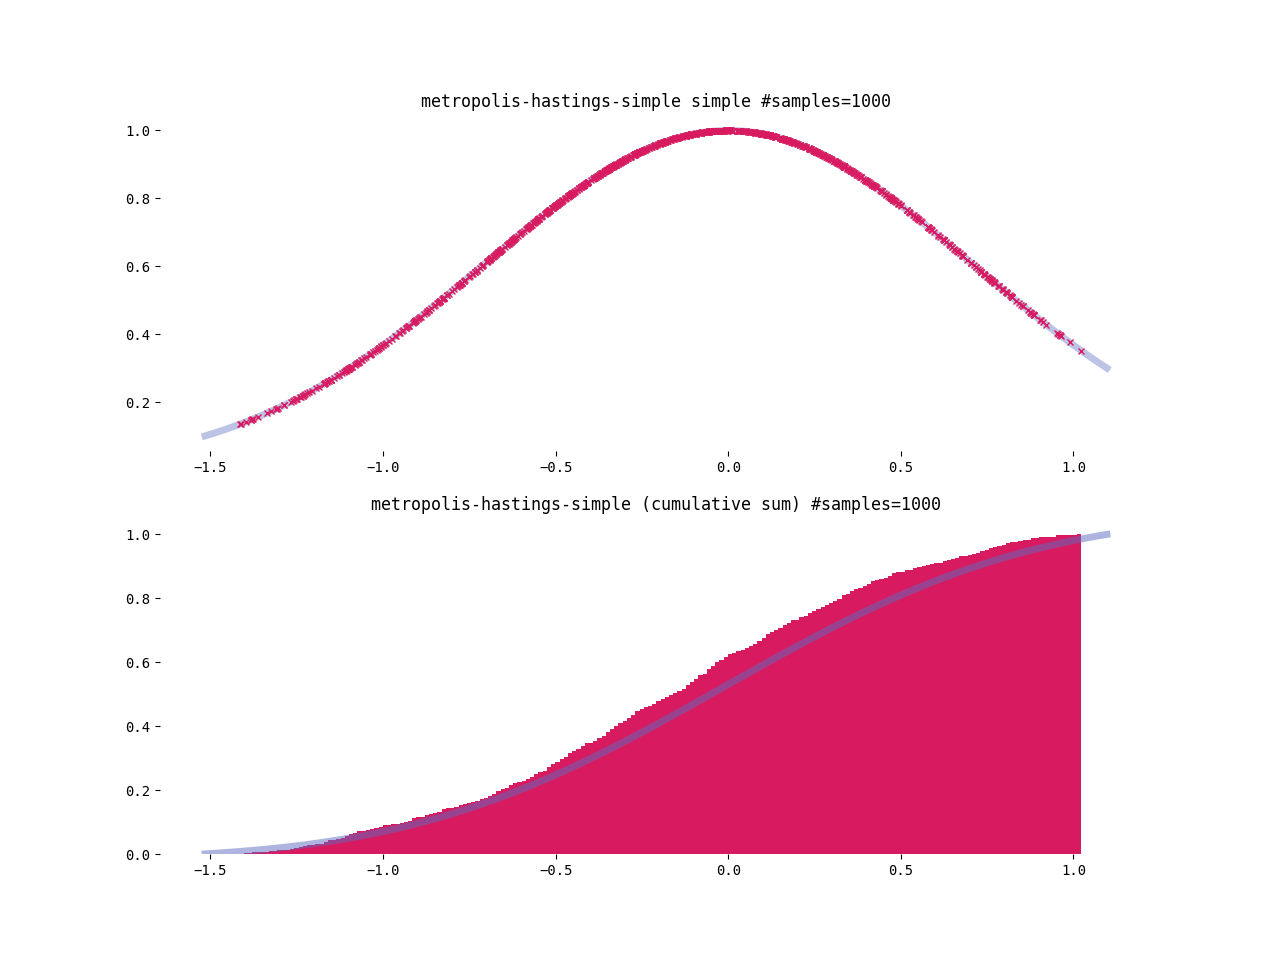
\includegraphics[width=\textwidth]{mcmc-mh-simple-1d-exp.png}

We can see from the plots of the raw samples and the cumulative distribution
that we wind up overshooting. This is because the markov chain, by definition,
has correlations between samples; However, we are supposed to be drawing
\emph{independent} samples from $\P$ for plotting/downstream use.

\subsubsection{Sampling per \texttt{iters\_per\_sample} steps}

The solution is to take samples that are \emph{spaced out} --- that is,
we do not consider each step from the markov chain as a sample. Rather,
we consider the state we are in after some \texttt{iters\_per\_sample} steps to be a sample.
In code, this is now:

{\footnotesize
\begin{minted}{py}
#  mcmc1d.py
def mh_uncorr(x0, prob, prop, iters_per_sample):
    yield x0; x = x0;
    while True:
        for i in range(iters_per_sample):
            xnext = prop(x); p = prob(x); pnext = prob(xnext)
            r = np.random.uniform() + 1e-5;
            if r < min(1, pnext/p): x = xnext
        yield xnext
...
def exp(x): return np.exp(-x*x)
def expprop(x): return np.random.normal(loc=x, scale=1e-1)
...
NSAMPLES = 1000; ITERS_PER_SAMPLE = 20
xs = list(itertools.islice(mhsimple(0, exp, expprop, ITERS_PER_SAMPLE), NSAMPLES))
\end{minted}
}

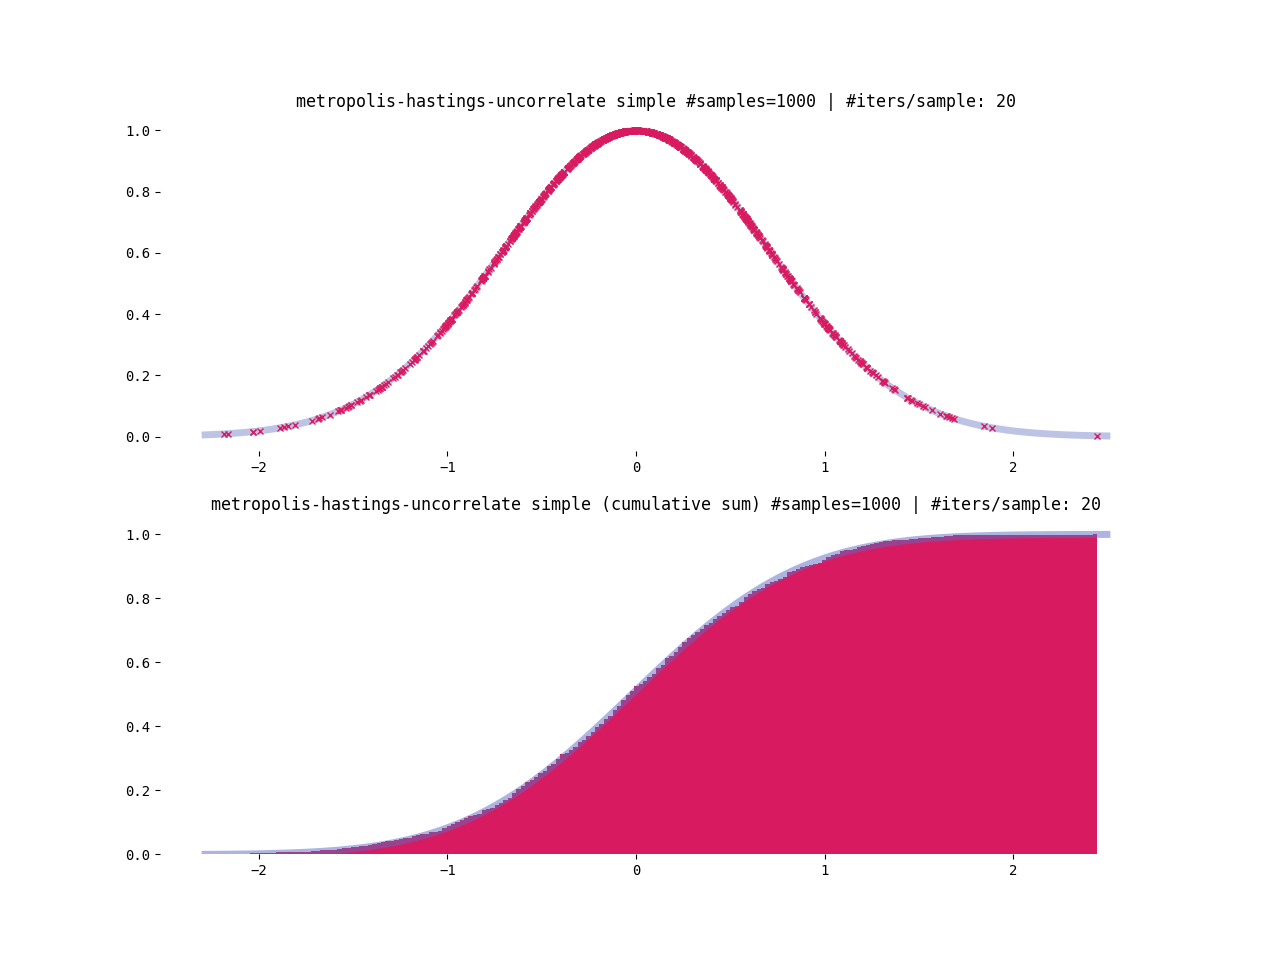
\includegraphics[width=\textwidth]{mcmc-mh-uncorr-1d-exp.png}

% \section{Gibbs sampling}
% We wish to sample from a joint distribution $P(X_1, X_2, X_3)$. However, it might
% be far cheaper to sample $P(X_1 | X_2, X_3)$, $P(X_2 | X_1, X_3)$, and
% $P(X_3 | X_1, X_2)$. If it is indeed cheaper, then we can use a Gibbs sampler
% to draw from the actual distribution $P(X_1, X_2, X_3)$ by combining samples
% from the \emph{conditional} distribution cleverly. The code is:
% 
% 
% \subsection{Gibbs sampling maintains detail balance}
% % https://stats.stackexchange.com/questions/118442/does-the-gibbs-sampling-algorithm-guarantee-detailed-balance
% Consider a two-variate state where we sample the first variable from its conditional distribution.
% A move between  $(x_1, x_2)$ and $(y_1, y_2)$ has zero probability in both directions
% if $x_2\neq y_2$, and thus detail balance automatically holds. If $x_2 = y_2$, then
% we can consider:
% 
% 
% \begin{align*}
% &\pi(x_1, x_2)  Prob((x_1, x_2) \rightarrow (y_1, x_2)) \\
% &= \pi(x_1, x_2) p(y_1 | X_2 = x_2) \\
% &= \pi(x_1, x_2) \frac{\pi(y_1, x_2)}{\sum_z \pi(z, x_2)} \\
% &= \pi(y_1, x_2) \frac{\pi(x_1, x_2)}{\sum_z \pi(z, x_2)} \quad \text{[move $(y_1, x_2)$ from the fraction outside]} \\
% &=\pi(y_1, x_2) p(x_1 | X_2 = x_2) \\
% &= \pi(y_1, x_2) Prob((y_1, x_2) \rightarrow (x_1, x_2))
% \end{align*}
% 
% \subsection{code}
% \begin{minted}{py}
% # sampler_x: y, z -> new x
% # sampler_y: x, z -> new y
% # sampler_z: x, y -> new z
% # N: number of iterations.
% # returns: a generator of the new (x, y, z)
% def sampler_xyz(sampler_x, sampler_y, sampler_z, x0, y0, z0, N):
%     (x, y, z) = (x0, y0, z0)
%     while True:
%       for i in range(N):
%         x = sampler_x(y, z)
%         y = sampler_y(x, z) # NOTE: use *new* x
%         z = sampler_z(x, y) # NOTE: use *new* x, y
%       yield (x, y, z)
% \end{minted}

\section{Hamiltonian Monte Carlo}
% https://www.cs.toronto.edu/~radford/ftp/ham-mcmc.pdf
% http://www.mcmchandbook.net/HandbookChapter5.pdf
% https://arxiv.org/pdf/1701.02434.pdf
% http://people.duke.edu/~ccc14/sta-663-2018/notebooks/S10E_HMC.html

If our target probability density $\P: X \rightarrow [0, 1]$ is \emph{differentiable},
then we can use the derivative of $\P(x)$ to provide better proposals. The idea
is as follows:

\begin{itemize}
    \item Interpret the probability landscape as a potential, with
        points of high probability being "valleys" and points of low probability
        being "peaks" (ie, invert the probability density with a transform
        such as $U[\P](x) = -\log \P(x)$. This way, a ball rolling on this
        terrain will try to move towards the valleys --- which are the locations
        of high probability $\P$.
    \item For a proposal at a position $x_0 \in X$, keep a ball at $x_0$,
        \emph{randomly choose its velocity}, simulate the ball according to 
        classical mechanics (Newton's laws of motion) for a fixed duration $D \in \R$
        and propose the final position as the final position of the ball. This
        is reversible and detail balanced because 
        \emph{classical mechanics is reversible and detail balanced}.
\end{itemize}

% \begin{align*}
%     &\frac{\partial \q}{\partial t} = \frac{\partial H}{\partial \p} \qquad
%     \frac{\partial \p}{\partial t} = - \frac{\partial H}{\partial \q} \\
%     &H(\q, \p) \equiv  U(\q) + K(\p) \\
%     &U(\q) \equiv \text{potential enetry} = - \log \P(\q) \quad K(\p) \equiv \text{kinetic energy} = \p^T \p/2
% \end{align*}

We wish to sample from a new distribution $P_H$, which is defined as:

\begin{align*}
&P_H[\P](\p, \q) \equiv \exp(-H[\P](\p, \q)) \qquad \text{(Sample states with low energy: Boltzmann/Ising model)}\\
&= \exp(-(U[\P](\q) + K(\p))) \qquad \text{(by defn. of hamiltonian, $H[\P] = U[\P] + K$)}\\
&= \exp(-(-\log \P(\q) + \p^T \p/2)) \qquad \text{(by choice of $U$ as NLL, $K$ as classical KE)}\\
&= \exp(\log \P(\q) - \p^T \p/2)) \\
&= \exp(\log \P(\q)) \cdot \exp(-\p^T \p/2) \\
&= \P(\q) \cdot \exp(-\p^T \p/2) \\
\end{align*}

Note that the probability distribution for $P_H[\P]$ has split into two
independent distributions: $\P(\q)$, and $\exp(-\p^T \p/2)$. Hence,
sampling $(\p, \q) \sim P_H[\P]$ correctly is \emph{equivalent} to 
sampling $\q \sim \P$, and $\p \sim \exp(-\p^T\p/2)$. Therefore, if we can
sample from $P_H$ effectively, taking only $(\q, \_) \sim P_H[\P]$ will
correctly give us the samples we are looking for.

We will show that using MCMC to sample from the $P_H[\P]$ above, with a particular
proposal function $\Prop_H$ that we shall define momentarily will provide
us with samples $(\p, \q)$ such that the $\q$ is sampled from $\P$.
This begs the question: "why do we need $\p$ anyway?" We will
show how introducing this $\p$ allows for rapid exploration of the space of possible
$\q$s.

\subsection{The proposal function for HMC}

In classical mechanics, once we have a hamiltonian $H(\q, \p)$, the dynamics of the
system are simulated according to the equations (called Hamilton's equations):
\begin{align*}
\frac{\partial \q}{\partial t} = \frac{\partial H[\P]}{\partial \p} \qquad
\frac{\partial \p}{\partial t} =  \frac{-\partial H[\P]}{\partial \q} 
\end{align*}

These equations, specialized to our situation become:

{\footnotesize
\begin{align*}              
    &\frac{\partial \q}{\partial t} 
      = \frac{\partial H[\P]}{\partial \p} 
      = \frac{\partial (U[\P](\q) + K(\p))}{\partial \p} 
      = \frac{\partial K(\p)}{\partial \p} 
      = \frac{\partial (\p^T \p)}{\partial \p} = 2\p \\
&\frac{\partial \p}{\partial t} 
    =  \frac{-\partial H[\P]}{\partial \q} 
    = \frac{-\partial (U[\P](\q) + K(\p))}{\partial \q}  
    = \frac{-\partial U[\P](\q)}{\partial \q}  
    =  \frac{-\partial -\log \P(\q)}{\partial \q} 
    =  \frac{\partial \log \P(\q)}{\partial \q}  \\
\end{align*}
}

We will denote a solution to the above system of equations as 
$(\q_{final}, \p_{final}) \equiv X_H[\P](\q_0, \p_0, T_0)$. That is, starting
from the position $(\p_0, \q_0)$, simulate the system for $T_0 \in \mathbb R$
time, according to Hamilton's equations. The final (position, momentum)
is $(\q_{final}, \p_{final})$.

Now, our proposal function will be:

$$
\Prop(\q_0, \_) \equiv \texttt{let } \p_0 \sim normal(0, 1) \texttt{ in } (X_H[\P](\q_0, \p_0, T_0)
$$

That is, we will  propose the new point as one obtained
from time evolution of the solutions to the hamiltonian; (a) we start from the
point $\q_0$; (b) pick a \emph{random velocity} $\p_0$; (c) simulate the
system for $T_0$ time using hamilton's equations; (d) return the final (position, momentum) as our proposal.

\subsection{Simulating the above regime}

\begin{minted}{py}
def euler(dhdp, dhdq, q, p, dt): % f(x + dx) = f(x) + f'(x) * dx
   pnew = p + -dhdq(q, p) * dt; qnew = q + dhdp(q, p) * dt
   return (qnew, pnew)


def hmc(q0, U, dU, nsteps, dt):
    # hamiltonian definition
    def h(q, p): return U(q) + 0.5*p*p
    def hdp(q, p): return  p
    def hdq(q, p): return dU(q)
    def nextsample(q, p): # run `euler` for n steps
        for _ in range(nsteps):
            (q, p) = euler(hdq, hdp, q, p, dt)
        return (q, p)

    yield q0; q = q0
    while True:
        p = np.random.normal(0, 1) # pick random momentum
        (qnext, pnext) = nextsample(q, p) # simulate next sample
        pnext = -p # reverse momentum so our process is reversible
        r = np.random.uniform(); # if accept according to MH, accept.
        if np.log(r) < h(q, p) - h(qnext, pnext): q = qnext
        yield q # return point
\end{minted}

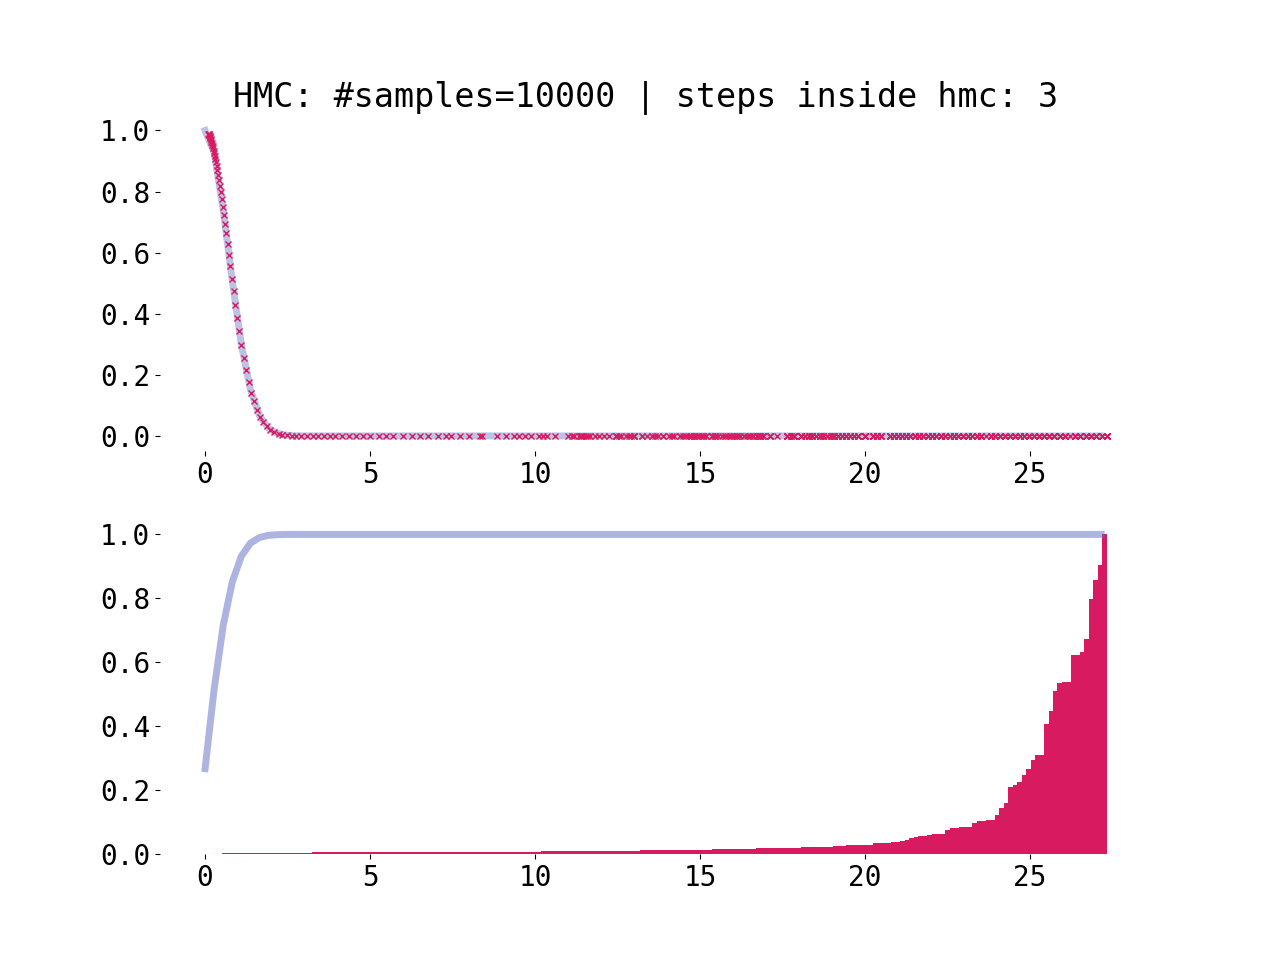
\includegraphics[width=\textwidth]{mcmc-hmc-WRONG-euler-1d-exp.png}
This has sampled disastrously: what is going wrong?

\subsection{Simulation: Euler integration}
Unfortunately, it turns out that running this simulation is in fact numerically
unstable on using a naive simulation schemes. For example, let us say
that we wish to simulate the orbit of a planet. Recall that we want
the proposal to be symmetric: so, if we simulate the trajectory of the planet
for $N$ timesteps, each timestep of time $\delta t$, and then \emph{reverse}
the momentum of the planet, run the next phse of the simulation for $N$ timesteps
with timestep $\Delta t$, we should begin where we started. However,
if we try to use the euler integration equations, here is what we see:

\begin{minted}{py}
def euler(dhdp, dhdq, q, p, dt):
   pnew = p + -dhdq(q, p) * dt
   qnew = q + dhdp(q, p) * dt
   return (qnew, pnew)
\end{minted}

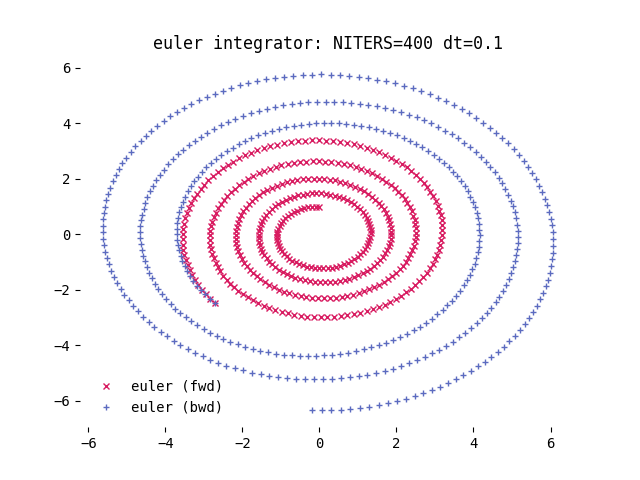
\includegraphics[width=\textwidth]{./euler-dt-0-1.png}

We can clearly see the forward trajectory (in pink) spiralling out, and
the backward trajectory (in blue), spiralling out even more. We can attempt
to fix this by making $\Delta t$ smaller:

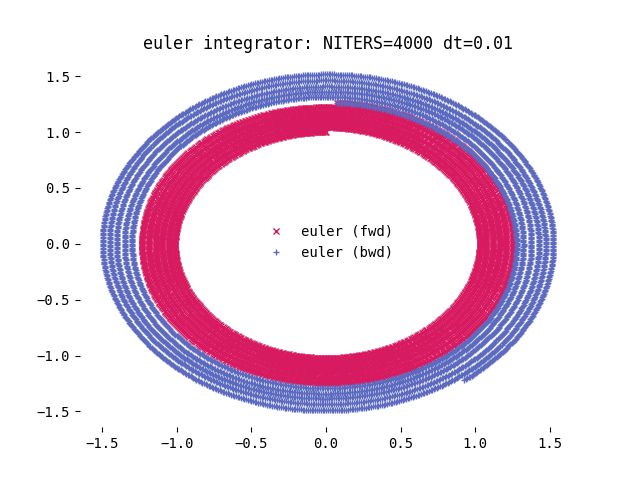
\includegraphics[width=\textwidth]{./euler-dt-0-01.png}


to no avail. Indeed, this is a \textbf{fundamental limitation of euler integration}.
Hence, we will need to explore more refined integration schemes.

\subsection{Simulation: Symplectic integrator}

The type of integrators that will allow us to get 'reasonable orbits' that
do not decay with time are knows as \emph{symplectic integrators}.
(An aside: the word \emph{symplectic} comes from Weyl, who substituted
the latin root in the word \emph{complex} by the corresponding greek root.
It is a branch of differential geometry which formalizes the consructs
needed to carry out hamiltonian mechanics on spaces that are more complicated
that Euclidian $\R^n$).

\begin{minted}{py}
## dq/dt = dH/dp|_{p0, q0}, dp/dt = -dH/dq|_{p0, q0}
def leapfrog(dhdp, dhdq, q0, p0, dt):
    p0 += -dhdq(q0, p0) * 0.5 * dt # kick: half step momentum
    q0 += dhdp(q0, p0) * dt # drift: full step position
    p0 += -dhdq(q0, p0) * 0.5 * dt # kick: half step momentum
    return (q0, p0)
\end{minted}


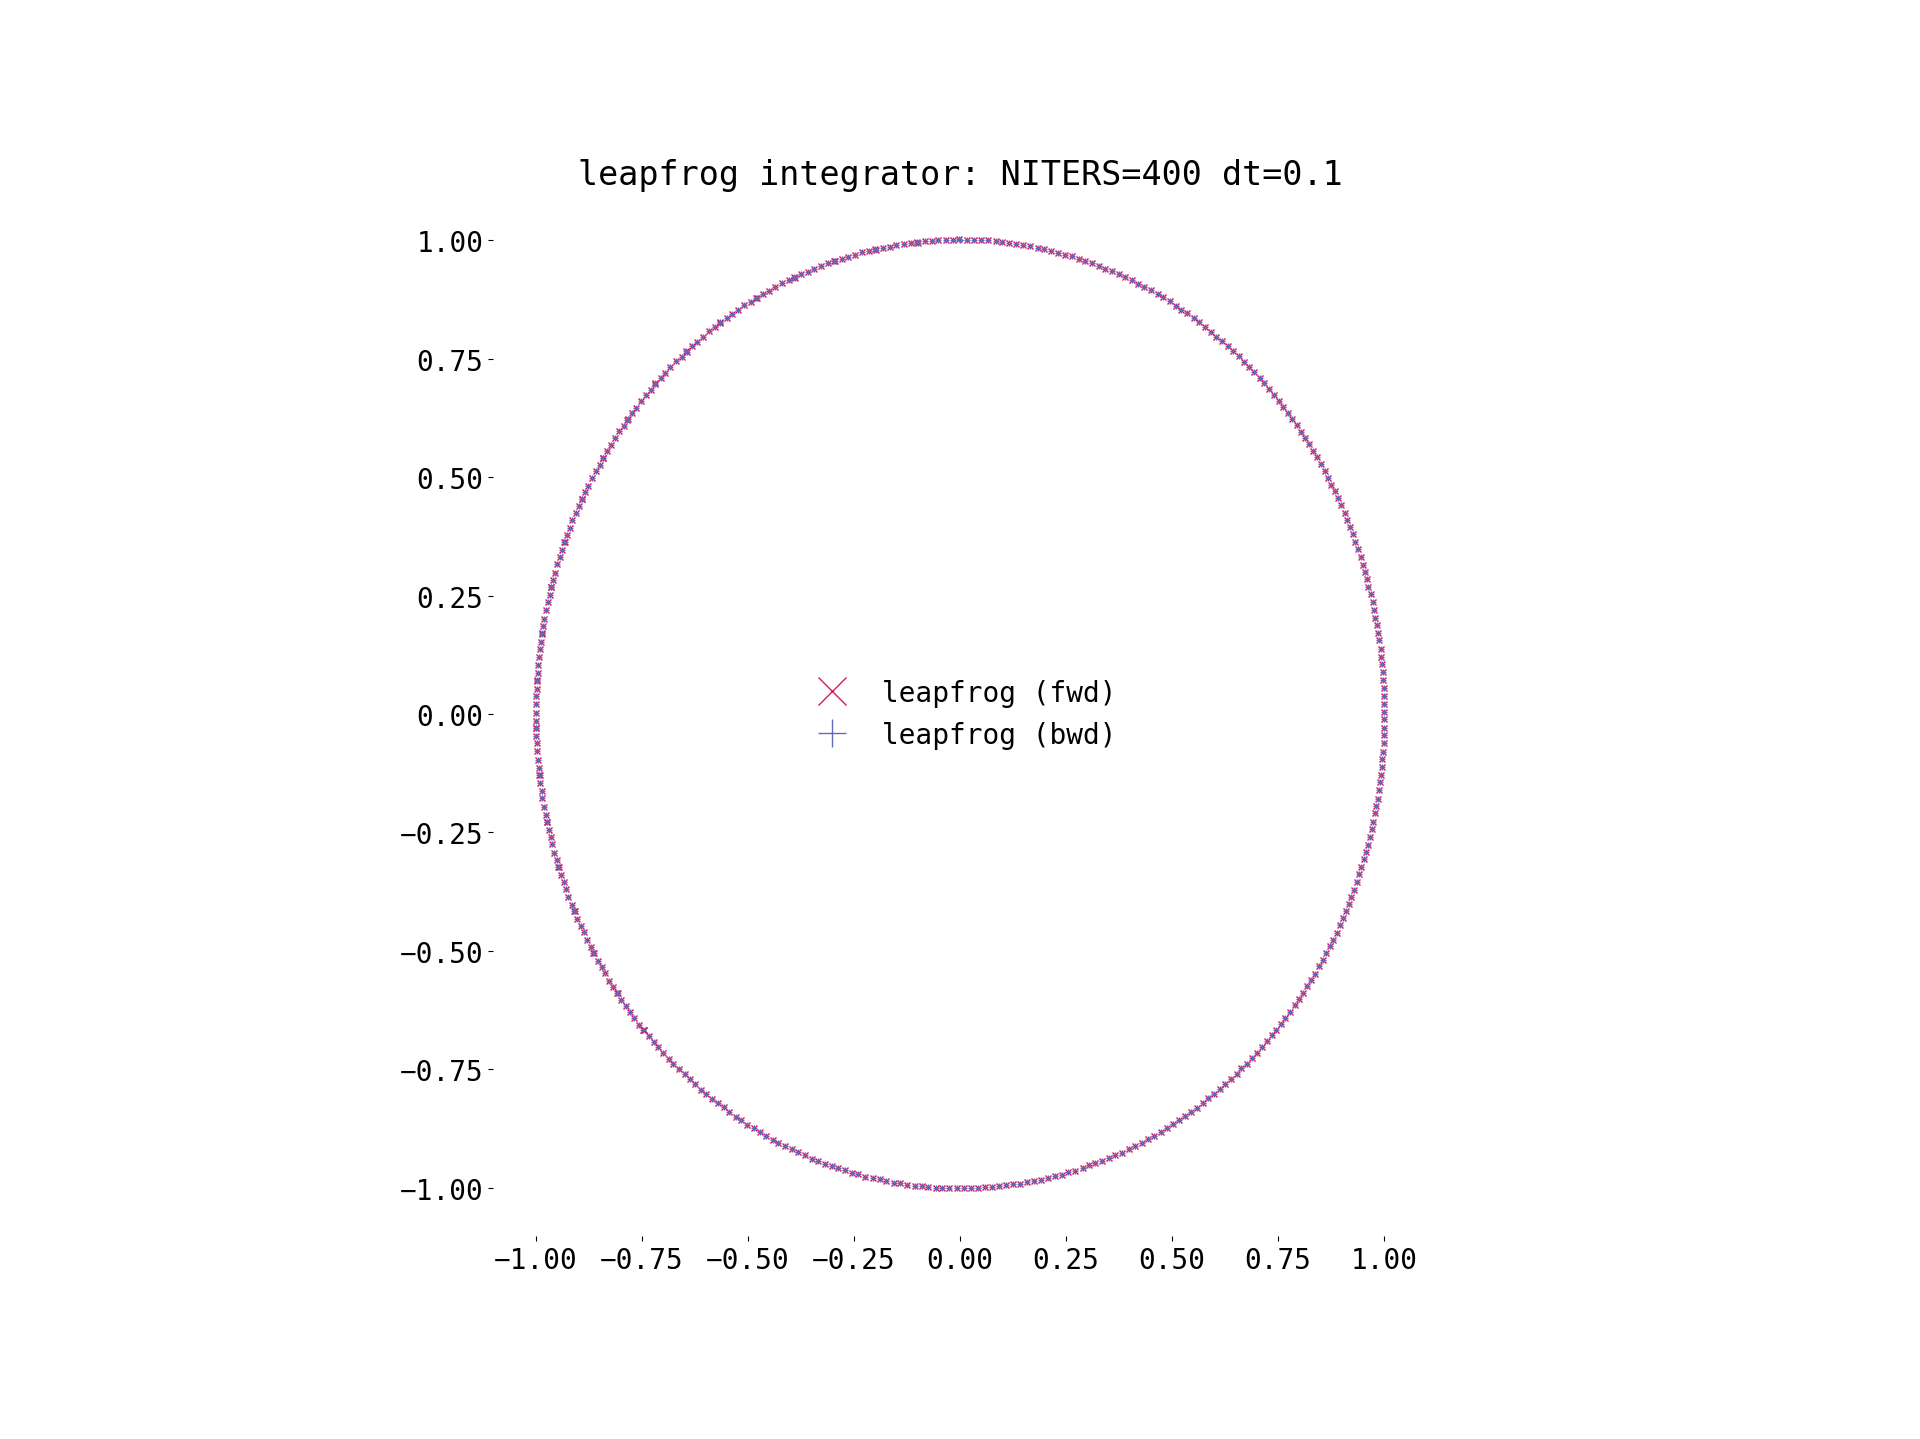
\includegraphics[width=\textwidth]{./leapfrog-dt-0-1.png}

It is clear from the plots that the leapfrog integrator is stable: orbits
stay as orbits. Indeed, we can prove the symplecticity/energy-preserving
property of this integrator.

\subsection{Proof that leapfrog is symplectic}
% http://physics.ucsc.edu/~peter/242/leapfrog.pdf

We will show that in phase space, the leapfrog integrator preserves infinitesimal
volumes of the form $dV \equiv d\p \times d\q$.


\subsection{Using HMC on the 1D gaussian}

Now that we have the math to setup a symmetric proposal distribution, let's
code up HMC on a 1D gaussian:

{\footnotesize

\begin{minted}{py}
def leapfrog(dhdq, dhdp, q0, p0, dt):
    p0 += -dhdq(q0, p0) * 0.5 * dt  # kick: half step momentum
    q0 += dhdp(q0, p0) * dt # drift: full step position
    p0 += -dhdq(q0, p0) * 0.5 * dt # kick: half step momentum
    return (q0, p0)

def hmc(q0, U, dU, nsteps, dt):
    def h(q, p): return U(q) + 0.5 * p*p
    def nextsample(q, p):
        for _ in range(nsteps):
            def hdp(q, p): return p
            def hdq(q, p): return dU(q)
            (q, p) = leapfrog(hdq, hdp, q, p, dt)
        return (q, p)

    yield q0; q = q0
    while True:
        p = np.random.normal(0, 1)
        (qnext, pnext) = nextsample(q, p)
        pnext = -p # reverse momentum so our process is reversible
        r = np.random.uniform(); 
        if np.log(r) < h(q, p) - h(qnext, pnext): q = qnext
        yield q
...
def neglogexp(x): return -1 * logexp(x)
def neglogexpgrad(x): return -1 * logexpgrad(x)
xs = list(take_every_nth(DECORRELATE_STEPS, 
    itertools.islice(hmc(1, neglogexp, neglogexpgrad, NSTEPS, DT), NSAMPLES*DECORRELATE_STEPS)))
\end{minted}
}

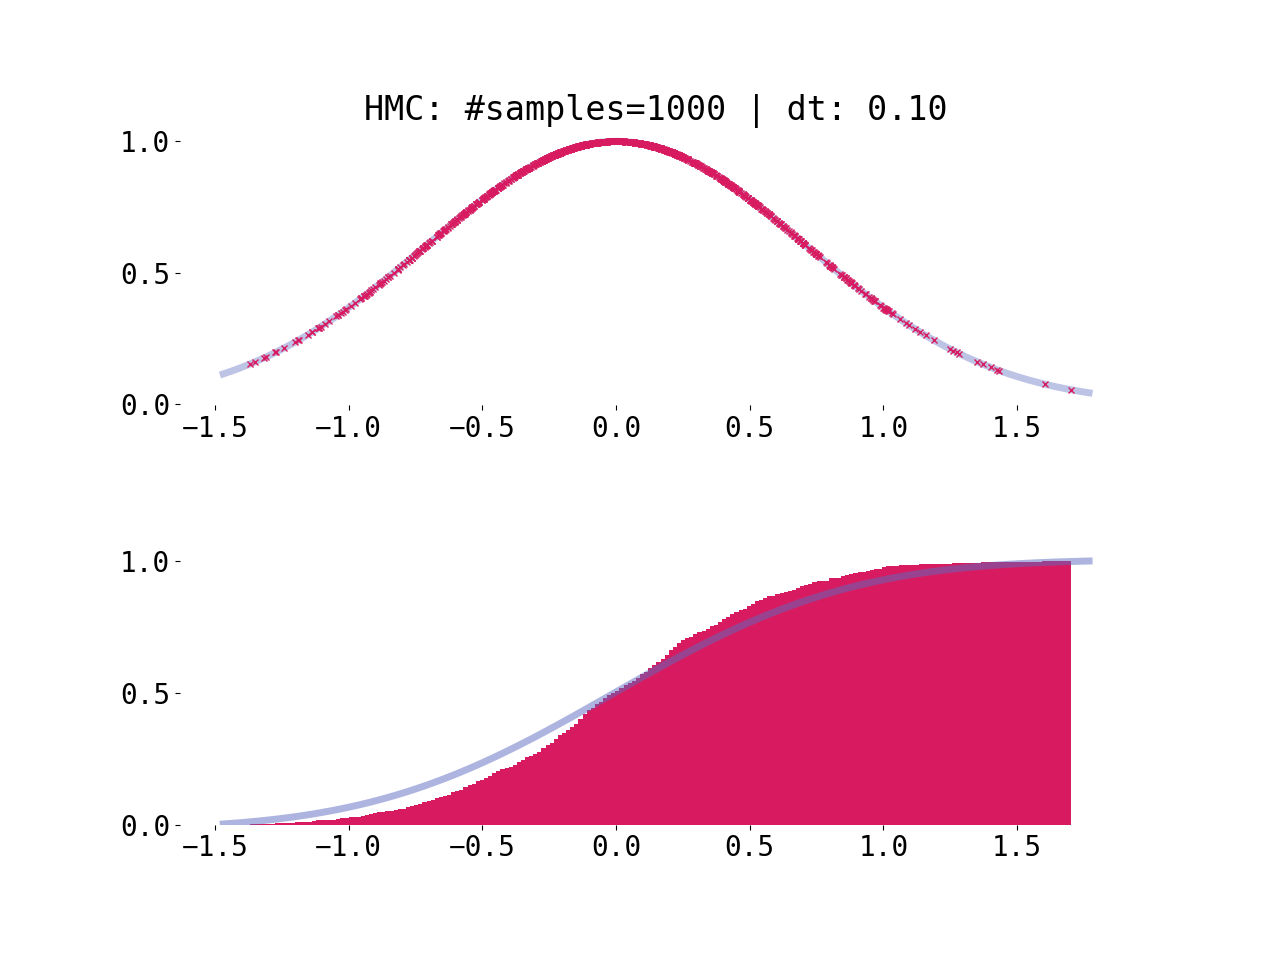
\includegraphics[width=\textwidth]{mcmc-hmc-1d-exp.png}

This looks far worse than the results we got from vanilla metropolis hastings:
why would anybody use this technique?


\subsection{HMC v/s MH when the proposal is atypical}

So far, I've hidden one thing under the rug: the \emph{initialization} of
the distribution. We've been starting at $x = 1$ --- let's now change that,
and start at $x = 600$. Note that this is very far from the "region of
interest" in the case of a standard normal distribution: 99\% of the probability
mass is in $[-3, 3]$ (the $3 \sigma$ rule).

\subsubsection{MH starting at $x = 600$}

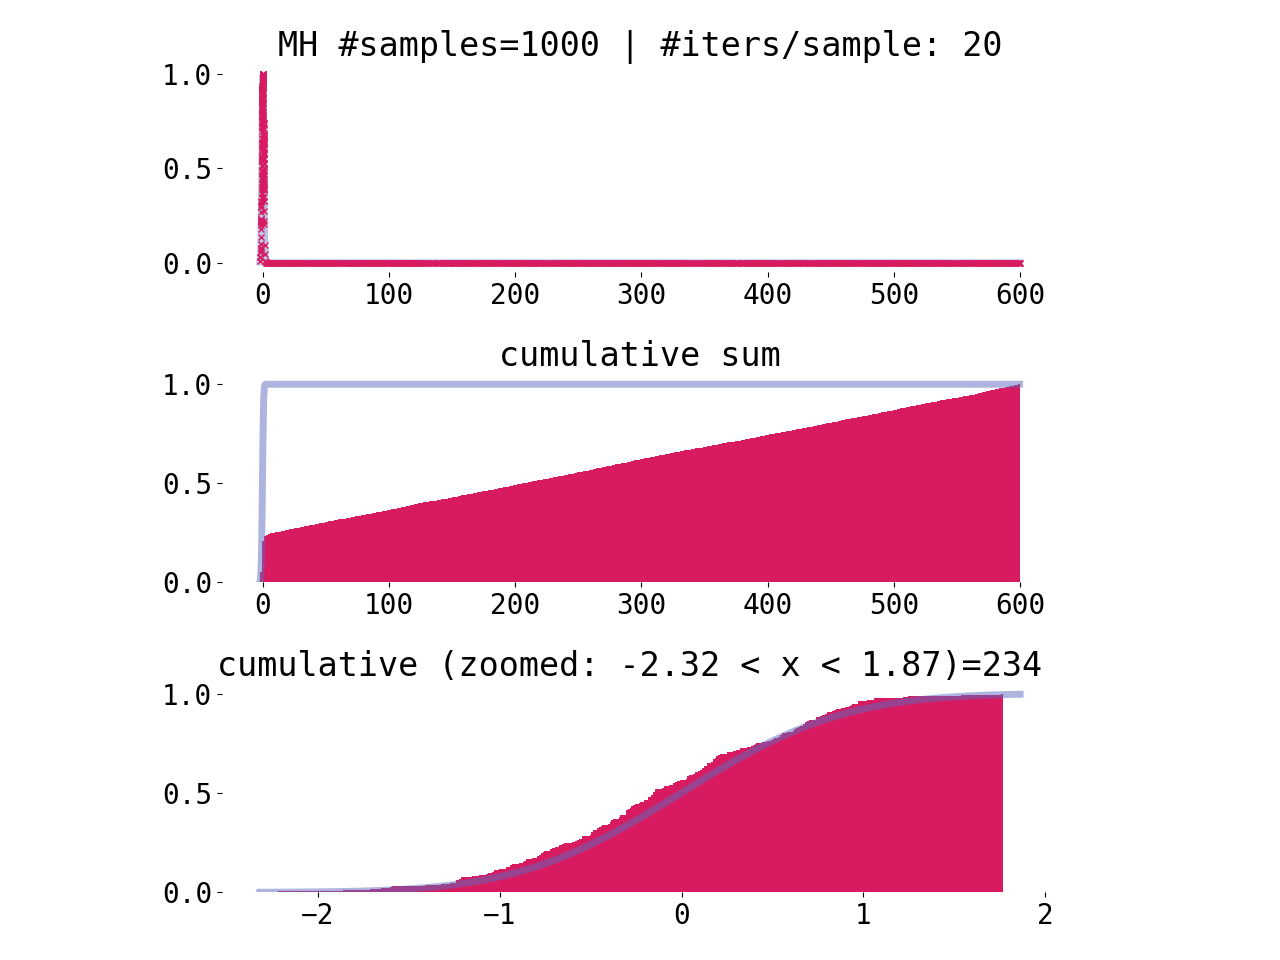
\includegraphics[width=\textwidth]{mcmc-mh-uncorr-1d-exp-startx-600.png}

Note that out of the $1000$ samples we started from, only $234$ are present
in the region of $-2 \leq x \leq 2$. We have wasted around $80\%$ of the
samples we have \emph{moving through the space} to get to the typical set.


\subsubsection{HMC starting at $x = 600$}

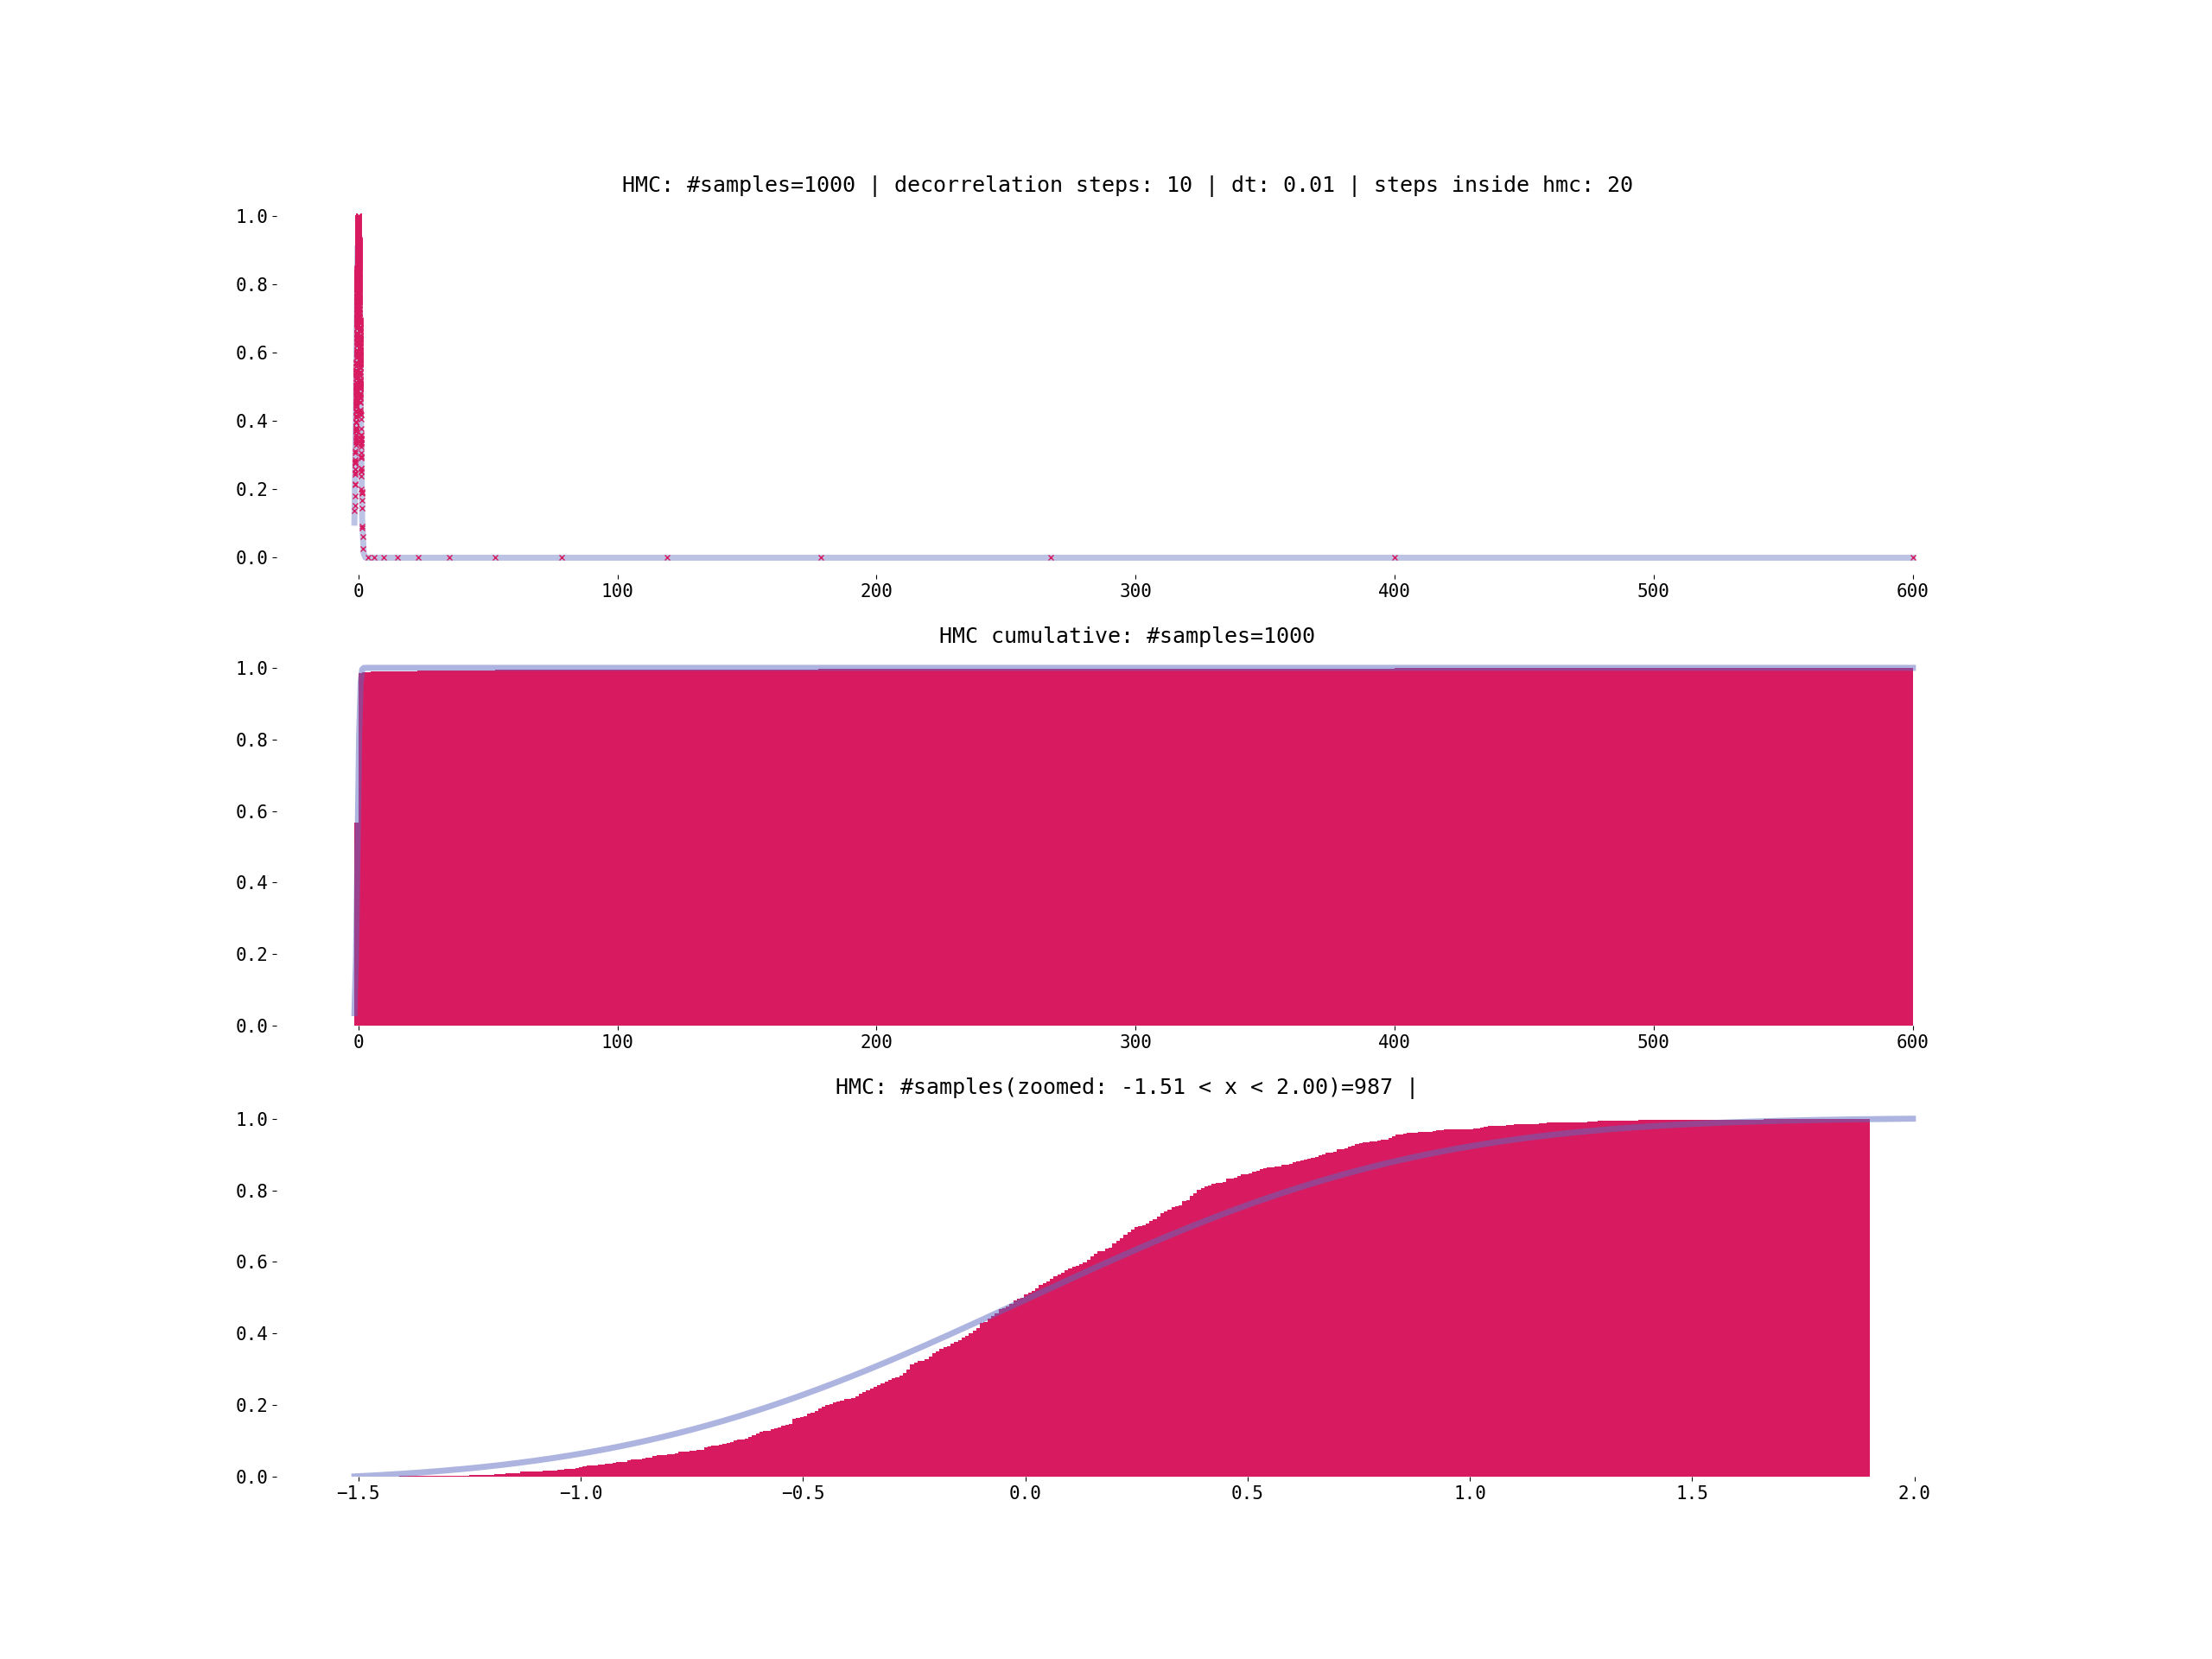
\includegraphics[width=\textwidth]{mcmc-hmc-1d-exp-startx-600.png}


Note that out of the $1000$ samples we started from, only $987$ are present
in the region of $-2 \leq x \leq 2$. Notice the distribution of samples
(pink crosses) in the hamiltonian monte-carlo case: most samples clustered around the gaussian;
our initial samples that are far away are powered by a strong potential energy
to move towards the center.

This is in stark contrast to the MH case, where the entire $x$-axis is pink,
due to the 'current point' having to move, proposal-by-proposal (which allows
at most a movement of distance $1$), from $600$ to $0$.


% \section{Discontinuous Hamiltonian monte carlo}
% 
% What if our distribution $P$ is \emph{discontinuouse}? How do we perform MCMC
% in that case?
% 
% \subsection{Hamilton's equations under laplace momntum}
% 
% \begin{align*}
%     \frac{d \q}{dt} = \m^{-1} \odot sign(\p) \qquad \frac{d \p}{dt} = - \nabla_q V(q)
% \end{align*}
% where $\odot$ is component-wise multiplication. If we know that $\p$ does
% not change sign, then our dynamics are correct; This is very different from
% the usual hamilton's equations, where we need to know the \emph{magnitude}
% of $\p$.
% 
% So, as long as we know that $\p$ has not changed sign, we can hold $sign(\p)$
% consant and use:
% 
% $$
% q(t + \epsilon) = q(t) + \epsilon m^{-1} \odot sign(\p(t))
% $$
% 
% Thus, we can jump across multiple discontinuities is $V(q)$ as long as we are
% aware that $sign(p(t))$ does not change.
% 
% TODO: write about the sudden drop in U when we cross a barrier.

% \section{Low discrepancy sequences}
% % https://cseweb.ucsd.edu/~dstefan/pubs/dalal:2008:low.pdf
% % https://openturns.github.io/openturns/master/theory/reliability_sensitivity/low_discrepancy_sequence.html
% Low discrepancy sequences are sequences of numbers that more evenly
% distributed than pseudorandom numbers in high dimensional space. Hence,
% simulations which use Low discrepancy sequences generally approximate
% integrals faster than psuedo-randomly generated points.
% 
% Formally, let us consider the $S$ dimensional half-open cube $\I^S \equiv [0, 1)^S$.
% assume we have a set of points $P \subseteq \I^S$, and a sub-interval
% $B \subseteq I^S$, where a sub-interval is a subset of the form 
% $B \equiv \prod_{i=1}^S \{ x \in \I : a_i \leq x \leq b_i \}$.
% 
% Given a universe set $X$ and two subsets $Large, Small \subseteq X$, we define
% the amount of containment of $Small$ in $Large$ to be $C(Small, Large) \equiv
% \frac{|Large \cap Small|}{|Large|}$. Intuitively, this measures the fraction
% of $Small$ that is in $Large$. We now define the discrepancy of the set
% of points $P$ relative to the sub-interval $B$ as:
% 
% \begin{align*}
% &D(B, P) \equiv \left| C(P, B) - C(B, \I^S) \right| \\
% &= \left| \frac{|B \cap P|}{|P|} - \frac{|B \cap \I^S|}{|\I^S|} \right|  \\
% &= \left| \frac{|B \cap P|}{|P|} - \frac{Volume(B)}{1} \right| \\
% &= \left| \frac{|B \cap P|}{|P|} - Volume(B) \right| \\
% \end{align*}
% 
% So, the discrepancy is measuring if $P$ fits within $B$ the way $B$ fits within
% the full space.
% 
% Now, the \textbf{worst-case-discrepancy} is defined as the maximum discrepancy
% over all sub-intervals:
% 
% $$
% D^\star(P) \equiv \max_{B \in \mathcal{J}} D(B, P)
% $$
% 
% where $\mathcal{J} \subseteq 2^{\I^S}$ is the set of all sub-intervals:
% 
% $$
% \mathcal{J} \equiv \{ \{ x \in \I^S : l[i] \leq x[i] \leq r[i]~\forall i \} : \vec l, \vec r \in \I^S \}
% $$
% 
% The goal is a \emph{low discrepancy sequence} is to minimise the worst-case-discrepancy.
% 
% \subsection{Error bounds for Numerical integration}
% 
% \subsection{Sobol sequences}
% 
% Sobol sequences are an example of low-discrepancy sequences
% 
% 
% \section{Future Work!}
% I've left the topic names up because they have interesting ideas, which I have
% sketched out in brief. Writing them down formally will take far too long; Hence,
% they've been left here [for the purposes of the project]. I will probably update
% this document even after the project, once I have grokked this material better.
% \section{Slice Sampling}
% 
% \section{No-U-Turn sampling}
% We no longer need to choose how many steps to walk with a no-U-turn-sampler.
% It prevents us from re-walking energy orbits, by detecting when we have completed
% traversing an orbit and are going to take a "U-turn". The details are quite
% complex, so we may not cover this here.

\end{document}

